\section{Robot and energy model}
\label{sec:robot-energy-model}

% WRITING PROMPTS (comments only; they do not print). About 2 pages. Consider
% renaming the section "Robot platform and energy model". Four parts.
%
% 1. The faculty robot as built (grey blocks in Fig. robot-architecture):
%    1200 x 800 mm steel frame, four 24 V / 250 W gear motors in skid steer,
%    L-faster dual motor driver, 24 V / 500 W / 6000 rpm blade motor through a
%    relay chain, EverExceed 25.6 V / 100 Ah LiFePO4 pack, driven by radio
%    (Microzone 6C-MINI with the MC7RB-V2 receiver: CH1 right, CH2 left, CH6
%    blade). Cite the faculty manuscript for these values.
% 2. The retrofit (blue blocks): what each added part does and why.
%    - Real-time controller between the receiver and the driver (Fig.
%      controller-wiring). Why keep the radio: the operator can always take
%      over, and a lost link stops the robot.
%    - The PWM relay module on the BLADE pulse. Its contacts (20 A at 14 V DC)
%      switch the coil of the blade contactor K1, not the 500 W blade current
%      (Fig. power-schematic). Explain this choice in one sentence.
%    - E-stop, bumper, RTK GNSS, IMU, battery V/I monitor, companion computer.
%    - The safety logic as a state machine (Fig. controller-states): ESTOP has
%      priority, then FAILSAFE, then the mode switch. Explain the re-arm rule
%      and why the bumper only latches in AUTO.
% 3. The energy model. Write the steady-state power terms (rolling, lateral
%    sliding moment, kinetic, efficiency, auxiliary): the formulas are in
%    src/lawn_mower_robot/lawn_mower_robot/energy.py. Then E_s(l) and
%    E_r(phi) for a straight from rest and an in-place turn (Fig. energy-model a, b).
%    Give the key comparison: 7.3 J/m straight, 24 J per 90 degree turn, so
%    one turn = 3.3 m of straight driving (placeholder robot).
% 4. Parameters: a table of the robot parameters with their source (measured,
%    datasheet, assumption). Say which are still placeholders and that the
%    results will be updated with the faculty robot.
%
% Ask yourself before submitting: are the fuse ratings, the DC-DC models and
% the controller board chosen? Put them in the parameter table or say they are
% typical parts.

\begin{figure*}[t]
\centering
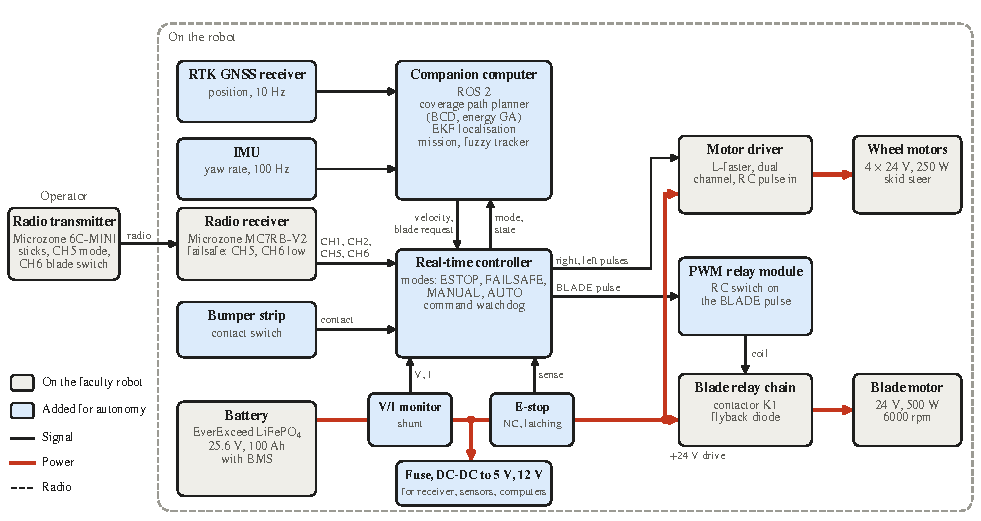
\includegraphics[width=\textwidth]{robot-architecture}
% DRAFT caption: rewrite in your own words.
\caption{Architecture of the robot. Grey blocks are on the faculty robot as built, which is driven by radio; blue blocks are added to make it autonomous. The real-time controller sits between the radio receiver and the actuators, so the operator can take over at any time.}
\label{fig:robot-architecture}
\end{figure*}

\begin{figure*}[t]
\centering
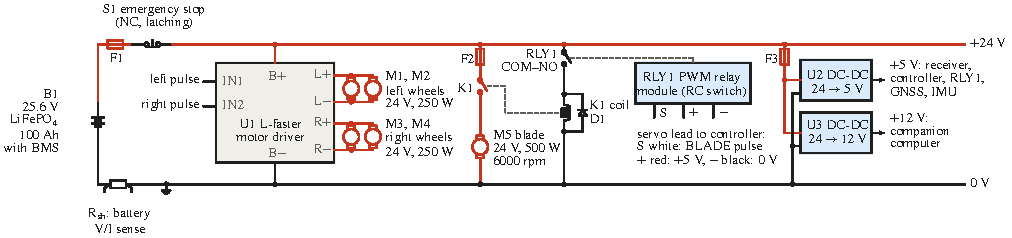
\includegraphics[width=\textwidth]{power-schematic}
% DRAFT caption: rewrite in your own words.
\caption{Power distribution. The emergency stop S1 cuts the 24~V drive bus: the motor driver, the blade and the coil of K1. The logic supply is taken before S1, so the controller stays powered and latches the stop. The PWM relay module RLY1 (relay SRA-05VDC-CL, contacts rated 20~A at 14~V~DC) is driven by the controller's BLADE pulse and switches the coil of the blade contactor K1, which carries the blade current. D1 is the flyback diode of the coil. Fuse ratings are left to the final wiring.}
\label{fig:power-schematic}
\end{figure*}

\begin{figure*}[t]
\centering
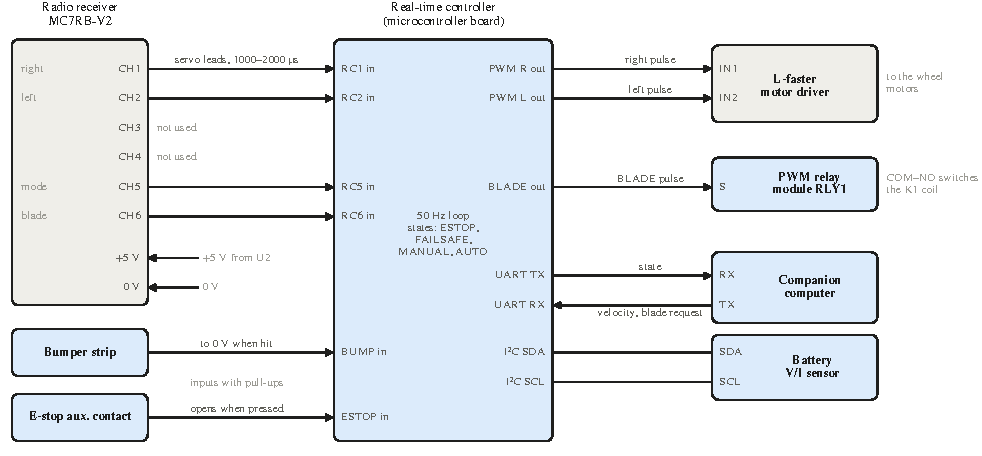
\includegraphics[width=\textwidth]{controller-wiring}
% DRAFT caption: rewrite in your own words.
\caption{Signal wiring of the real-time controller. It reads four receiver channels, the bumper and the emergency-stop contact, writes the drive pulses of the motor driver and the BLADE pulse of the PWM relay module, and exchanges commands and state with the companion computer.}
\label{fig:controller-wiring}
\end{figure*}

\begin{figure}[t]
\centering
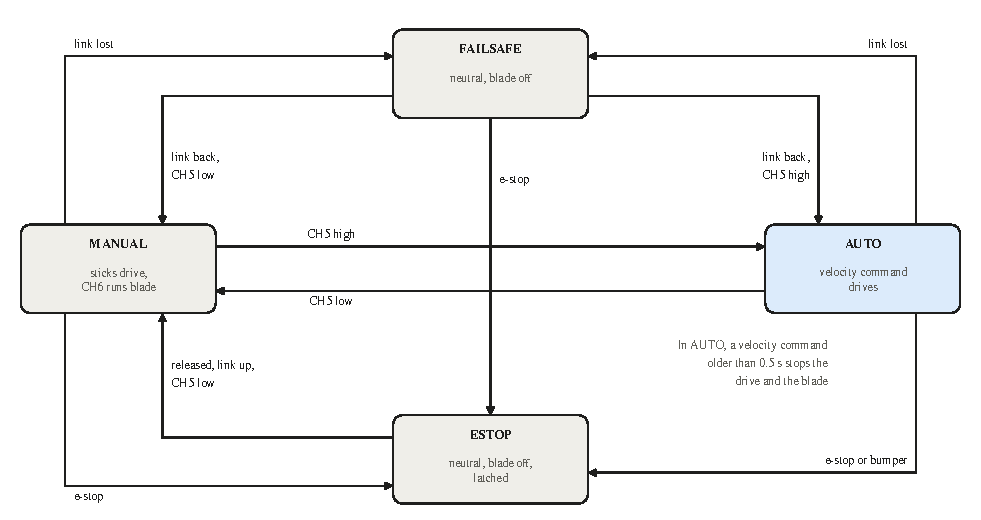
\includegraphics[width=0.7\textwidth]{controller-states}
% DRAFT caption: rewrite in your own words.
\caption{States of the real-time controller. The emergency stop has priority over a lost radio link, which has priority over the mode switch CH5. Only AUTO (blue) follows the companion computer.}
\label{fig:controller-states}
\end{figure}

\begin{figure*}[t]
\centering
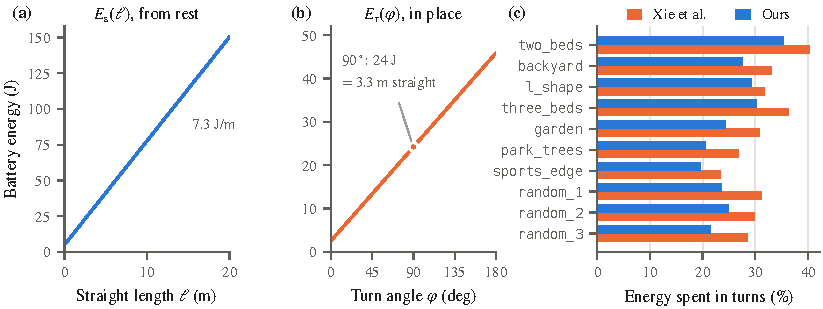
\includegraphics[width=\textwidth]{energy-model}
% DRAFT caption: rewrite in your own words.
\caption{Energy model of the placeholder robot (Pioneer 3-AT parameters). (a) Battery energy of a straight drive from rest. (b) Battery energy of a turn in place; a 90$^\circ$ turn costs as much as 3.3~m of straight driving. (c) Share of the plan energy spent in turns, for the plans of seed 0.}
\label{fig:energy-model}
\end{figure*}
